\documentclass[11pt, oneside]{article}
\usepackage[margin=1in,letterpaper]{geometry}
\usepackage{times}
\usepackage{graphicx}
\usepackage{amssymb,amsmath}
\usepackage{array}
\usepackage{longtable}
\usepackage{color}
\usepackage[T1]{fontenc}
\usepackage{sectsty}
\usepackage{tikz}
\usetikzlibrary{decorations.markings,calc,patterns}
\usepackage{pgfplots}
\pgfplotsset{compat=1.17}
\sectionfont{\fontsize{12}{12}\selectfont}
\subsectionfont{\fontsize{11}{11}\selectfont}
\subsubsectionfont{\normalsize\itshape\mdseries}

\renewcommand\labelitemi{{\boldmath$\cdot$}}

%%%%%%%%%%%%%%%%%%%%%%%%%%%%%%%%%%%%%
% Notation: unit vectors are \hat{\mathbf{k}}, etc. Symbols follow ../variables_master.tex.
% Renames that apply existing instructor decisions (each also marked at first use):
%   - EM wavenumber K_EM -> k and unit vectors \hat{K}_i, \hat{K}_r -> \hat{k}_i, \hat{k}_r (D14);
%   - EM wavelength lambda_EM -> lambda; water-surface wavelengths (handwritten lambda = 2 pi/K, lambda_Bragg) -> Lambda,
%     Lambda_Bragg (D61: Lambda is the wavelength of surface undulations);
%   - phase velocity v_p -> u_p (D15);
%   - surface tension gamma -> gamma_st (D9 reserves gamma for the propagation constant; the subscript follows the
%     D18 precedent tau -> tau_rel). Approved (D66);
%   - the local incidence angle theta_m -> theta_i' (the master-table symbol for the angle of incidence measured from
%     the local normal, L7; D57). Approved (D74).
% Instructor decisions (2026-09-29, master table D64--D75): kept as handwritten (approved): ocean wavenumber K,
% ocean angular frequency omega, surface tension gamma_st, GMF coefficients A, a, b, n, scattering coefficients
% alpha_pp, theta_i' (handwritten theta_m), mass density rho_w. Renamed (resolved): frequency spectrum Lambda(omega)
% -> Psi(omega) (D67); wind speed u_w -> U (D68); wind angle alpha -> phi_wind (D69); anti-plane tilt xi -> zeta
% (D72); tilted-patch reflectivities Gamma_pq -> |S_pq|^2 (D73).
% Main reference checks: Ulaby & Long (2014), pp. 428, 783-798, 868-869; van Zyl (2011), pp. 160, 198-201.
%%%%%%%%%%%%%%%%%%%%%%%%%%%%%%%%%%%%%

\title{Ge 158 Lecture 8: Scattering from the Ocean and Other Surfaces with Small-Scale Roughness}
\author{Brent Minchew}
\date{}

\setlength{\emergencystretch}{1.5em}
\begin{document}
\maketitle

\noindent\underline{\textbf{Topics covered}}
\begin{itemize}
	\item Ocean wave spectra
	\item Scattering from slightly rough surfaces (Bragg scattering)
	\item Scattering from undulating, slightly rough surfaces
\end{itemize}

%%%%%%%%%%%%%%%%%%%%%%%%%%%%%%%%%%%%%
\section{Overview}

\begin{itemize}
	\item We will use scattering of EM waves from the ocean surface as an illustrative example of scattering from a broad range of natural surfaces.
	\item Advantages of doing so:
	\begin{itemize}
		% NOTE: added "(Lecture 1)".
		\item allows us to incorporate concepts from the beginning of the semester on dielectric properties (Lecture 1), because temperature and salinity have important effects on scattering from the ocean;
		\item nicely illustrates the influence of surface roughness of varying wavelengths and sources.
	\end{itemize}
	\item To get started, let us consider the geometry of the surface and the processes that influence it.
\end{itemize}

%%%%%%%%%%%%%%%%%%%%%%%%%%%%%%%%%%%%%
\section{The ocean surface}
\label{s:ocean}

\subsection{What sets the elevation of the ocean surface}

\begin{itemize}
	\item The elevation of the ocean surface is influenced by a variety of factors. Roughly in order of decreasing wavelength:
	\begin{itemize}
		\item the gravitational equipotential surface (geoid), which approximates mean sea level and is the elevation that the ocean would take given a planet's mass distribution and rotation, and in the absence of external forcing (tides, winds, etc.);
		\item tides;
		\item atmospheric pressure gradients;
		\item currents;
		% NOTE: the handwritten mark beside this bullet is the same glyph as the star in the Lecture 7 notes
		% ("* Note: A_rs is not ...", written \bigstar there).
		\item[$\bigstar$] wind-driven waves $\rightarrow$ of greatest interest in today's lecture.
	\end{itemize}
\end{itemize}

\subsection{Wind-driven surface waves}

\begin{itemize}
	\item Ocean surface waves are mechanical waves that exist at the ocean--atmosphere boundary.
	\item As with any mechanical wave, they are defined by a perturbing force and a restoring force.
	\item In all cases of interest in this lecture, the perturbing forces are shear stresses caused by the wind.
	\item We will focus our attention on two types of waves defined by different restoring forces:
	\begin{enumerate}
		\item Gravity waves are long wavelength ($>2$~cm) whose restoring force is gravity.
		\begin{itemize}
			\item Swells, which build up from wind forcing over long timescales, are examples of gravity waves.
			\item Can play an important role in scattering from the ocean surface.
			\item Terrestrial analogs: rolling hills, crop rows.
		\end{itemize}
		% NOTE: the 2 cm boundary is where the gravity and surface-tension terms of the dispersion relation
		% (Eq. e:disp) are equal: K = sqrt(rho_w g/gamma_st) = 367 rad/m, i.e., Lambda = 1.71 cm (python3, with
		% gamma_st = 0.0728 N/m, rho_w = 1000 kg/m^3, g = 9.81 m/s^2). U&L 2014, p. 787, use a different naming
		% (capillary waves "a centimeter or less", capillary-gravity waves 1 cm to ~1 m).
		\item Capillary waves are short wavelength ($<2$~cm) whose restoring force is surface tension.
		\begin{itemize}
			\item Produce small-scale roughness that is superimposed on longer-wavelength roughness.
			\item Play a leading role in EM scatter from the ocean surface.
			\item Terrestrial analog is any small-scale roughness: rocks, small erosional features.
		\end{itemize}
	\end{enumerate}
	\item At radar wavelengths, it is often the case that the portion of the wave spectrum of greatest interest lies at intermediate wavelengths.
	\item At these intermediate wavelengths, both gravity and surface tension act to restore the ocean surface $\rightarrow$ such waves are called gravity--capillary waves.
\end{itemize}

\subsection{Dispersion relation for gravity--capillary waves}

% NOTE: handwritten K (ocean-wave wavenumber), omega, and rho_w kept (master table D64, D65, D75); handwritten gamma (surface
% tension) written gamma_st (D9, D66). Checked against the standard deep-water dispersion relation; in the limits it
% reduces to U&L 2014, Eqs. 17.5 (tanh KD -> 1 in deep water) and 17.6 (p. 869; B = gamma_st/rho_w = 73 cm^3/s^2),
% without their current term K_hat . U.
\begin{itemize}
	\item The dispersion relation for gravity--capillary waves in deep water (depth $\gg$ wavelength) is given as
	\begin{equation}
		\label{e:disp}
		\omega^2 = gK + \frac{\gamma_\mathrm{st}}{\rho_w}K^3,
	\end{equation}
	where
	\begin{itemize}
		\item $g \equiv$ gravitational acceleration;
		\item $\gamma_\mathrm{st} \equiv$ surface tension;
		\item $\rho_w \equiv$ mass density of water;
		% NOTE: added the definitions of omega and K (the handwriting uses them without definition), and "(= 2 pi/Lambda)".
		\item $\omega \equiv$ angular frequency and $K \equiv$ wavenumber ($= 2\pi/\Lambda$) of the ocean-surface wave.
	\end{itemize}
	% NOTE: handwritten "approx" written "->" for the limits (instructor preference); handwritten rho (no subscript)
	% in the large-K limit written rho_w.
	\item In the limits
	\begin{itemize}
		\item small $K$: $\omega \rightarrow \sqrt{gK}$ for gravity waves;
		% NOTE: added "for capillary waves", parallel to the small-K line.
		\item large $K$: $\omega \rightarrow \sqrt{\gamma_\mathrm{st}K^3/\rho_w}$ for capillary waves.
	\end{itemize}
	\item We can see from this expression how ``surfactants'' (substances that reduce surface tension) change the dispersion relation of ocean surface waves $\Rightarrow$ change the scattering properties of EM waves.
	\item Common examples of surfactants include mineral oil (as in the oil spill example that we have seen many times so far in this course) and biological films. Microplastics may also act as a surfactant, but I believe this remains an open question.
\end{itemize}

\subsection{Phase velocity}

% NOTE: interpretive item for the instructor. The equilibrium statement below is kept as handwritten. For the
% Pierson-Moskowitz spectrum (Eq. e:PM) the phase speed at the spectral peak, g/omega_peak, is 1.14 U (python3),
% so "wave speed ~ wind speed" holds for the dominant gravity waves of a fully developed sea; it cannot hold for
% cm-scale gravity-capillary waves, whose phase speed is at most a few tens of cm/s near the minimum
% u_p,min = (4 g gamma_st/rho_w)^(1/4) = 0.23 m/s.
\begin{itemize}
	% NOTE: handwritten v_p written u_p (master table D15); handwritten rho written rho_w.
	\item Gravity--capillary waves are excited (grow) in a turbulent wind field and reach equilibrium when the wind speed matches the phase velocity of the surface waves. From the dispersion relation, we define the phase velocity
	\begin{equation}
		\label{e:up}
		u_p = \frac{\omega}{K} = \sqrt{\frac{g}{K} + \frac{\gamma_\mathrm{st}}{\rho_w}K}.
	\end{equation}
	\item In general, surfactants will reduce the surface tension of clean water $\Rightarrow$ (all else being equal) will slow (gravity--)capillary waves (Figure~\ref{f:up}).
	% NOTE: added "(Figure~\ref{f:up})".
\end{itemize}

\begin{figure}[!htbp]
	\centering
	% Reproduces the handwritten sketch (page L5): axes u_p (handwritten v_p) vs. wavelength (handwritten
	% "lambda (= 2 pi/k)", written Lambda (= 2 pi/K), D61); two solid gravity-capillary curves (gamma_1 above,
	% gamma_2 below, converging at long wavelength); one dashed gravity-wave asymptote (rising from the origin, the
	% same for both); two dotted capillary asymptotes (gamma_1 above gamma_2, decreasing with wavelength); labels as
	% handwritten. Curves from Eq. (e:up) with K = 2 pi/Lambda: gamma_st,1 = 0.0728 N/m (clean water, 20 C) and
	% gamma_st,2 = 0.035 N/m (illustrative surfactant-covered water), rho_w = 1000 kg/m^3, g = 9.81 m/s^2.
	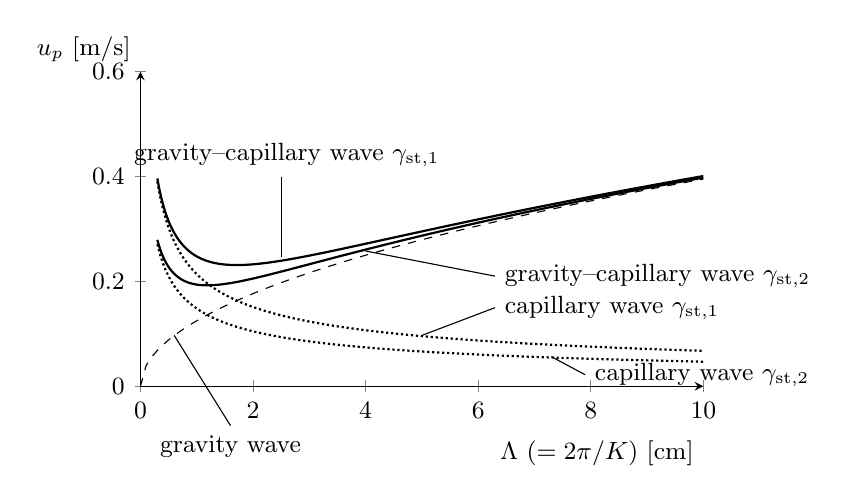
\begin{tikzpicture}
		\begin{axis}[
			width=0.72\textwidth, height=0.46\textwidth,
			axis lines=left, xmin=0, xmax=10, ymin=0, ymax=0.6,
			xlabel={$\Lambda\ (=2\pi/K)$ [cm]}, ylabel={$u_p$ [m/s]},
			every axis x label/.style={at={(current axis.right of origin)},anchor=north east, yshift=-16pt},
			every axis y label/.style={at={(current axis.above origin)},anchor=south east},
			clip=false, font=\small, ymax=0.6, restrict y to domain=0:0.62,
			]
			\def\g{9.81}\def\ga{0.0728}\def\gb{0.035}
			% gravity-capillary waves
			\addplot[thick, samples=300, domain=0.3:10] {sqrt(\g*x/100/(2*pi) + 2*pi*\ga/(1000*x/100))};
			\addplot[thick, samples=300, domain=0.3:10] {sqrt(\g*x/100/(2*pi) + 2*pi*\gb/(1000*x/100))};
			% gravity-wave asymptote
			\addplot[dashed, samples=100, domain=0:10] {sqrt(\g*x/100/(2*pi))};
			% capillary asymptotes
			\addplot[densely dotted, thick, samples=200, domain=0.3:10] {sqrt(2*pi*\ga/(1000*x/100))};
			\addplot[densely dotted, thick, samples=200, domain=0.3:10] {sqrt(2*pi*\gb/(1000*x/100))};
			% labels with leaders to the curves (curve values from Eq. e:up, python3)
			\node[anchor=south] at (axis cs:2.6,0.40) {gravity--capillary wave $\gamma_{\mathrm{st},1}$};
			\draw (axis cs:2.5,0.40) -- (axis cs:2.5,0.246);
			\node[anchor=west] at (axis cs:6.3,0.21) {gravity--capillary wave $\gamma_{\mathrm{st},2}$};
			\draw (axis cs:6.3,0.21) -- (axis cs:4.0,0.258);
			\node[anchor=west] at (axis cs:6.3,0.15) {capillary wave $\gamma_{\mathrm{st},1}$};
			\draw (axis cs:6.3,0.15) -- (axis cs:5.0,0.097);
			\node[anchor=west] at (axis cs:7.9,0.022) {capillary wave $\gamma_{\mathrm{st},2}$};
			\draw (axis cs:7.9,0.022) -- (axis cs:7.3,0.0565);
			\node[anchor=north] at (axis cs:1.6,-0.075) {gravity wave};
			\draw (axis cs:1.6,-0.075) -- (axis cs:0.6,0.097);
		\end{axis}
	\end{tikzpicture}
	\caption{Phase velocity of deep-water gravity--capillary waves (solid, Eq.~\ref{e:up}) versus wavelength for clean water ($\gamma_{\mathrm{st},1} = 0.0728$~N/m) and for water whose surface tension has been reduced by a surfactant ($\gamma_{\mathrm{st},2} = 0.035$~N/m, illustrative). Dashed: gravity-wave limit $\sqrt{g/K}$; dotted: capillary-wave limits $\sqrt{\gamma_\mathrm{st}K/\rho_w}$.}
	\label{f:up}
\end{figure}
% NOTE: the caption and the numerical values of gamma_st are added.

\subsection{Wave height, the wave spectrum, and wind}

\begin{itemize}
	% NOTE: handwritten Lambda(omega) (frequency spectrum) written Psi(omega) (D67) and handwritten u_w (wind speed)
	% written U (D68), as in Ulaby & Long.
	% Eq. (e:h2) agrees with U&L 2014, Eq. 17.7 (p. 869), where the frequency spectrum is S(Omega).
	\item When wave speed (phase velocity) matches wind speed, the RMS height $h$ of the ocean can be defined as
	\begin{equation}
		\label{e:h2}
		h^2 = \int_0^\infty \Psi(\omega)\,d\omega,
	\end{equation}
	% NOTE: handwritten reads Lambda(omega) = g^2/(10 omega^5) exp{-3/4 (g/(u_w omega))^4}; corrected the
	% coefficient 1/10 to 8.1e-3 because this is the Pierson-Moskowitz (1964) spectrum for a fully developed sea
	% (the spectrum plotted in U&L 2014, Fig. 17-5, p. 868, which gives no formula), whose constants are
	% alpha = 8.1e-3 and beta = 0.74 (kept as the handwritten 3/4), with U the wind speed 19.5 m above the sea
	% surface. Check (python3): Eq. (e:h2) gives h^2 = alpha U^4/(4 beta g^2); at U = 10 m/s the handwritten
	% coefficient gives h = 1.86 m (significant wave height 4h = 7.4 m, U&L p. 869), 12 times the variance of the
	% Pierson-Moskowitz value h = 0.53 m (4h = 2.1 m). The constants are from Pierson & Moskowitz (1964), which is not
	% in the course texts. Added "(measured 19.5 m above the sea surface)".
	where the frequency spectrum $\Psi$ is related to the local wind speed $U$ (measured 19.5~m above the sea surface) through the empirical relation
	\begin{equation}
		\label{e:PM}
		\Psi(\omega) = \frac{8.1\times10^{-3}\,g^2}{\omega^5}\exp\left\{-\frac{3}{4}\left(\frac{g}{U\omega}\right)^4\right\}
	\end{equation}
	$\Rightarrow$ strong correlation between wind speed and surface height, which, of course, we all know from experience.
	% NOTE: added "(the Pierson--Moskowitz spectrum for a fully developed sea)".
	(Eq.~\ref{e:PM} is the Pierson--Moskowitz spectrum for a fully developed sea.)
	\item For remote sensing, we are concerned with the direction of the winds relative to the look direction (or plane of incidence of the EM wave) of the sensor. This relation is usually given as an empirical relation between the normalized radar cross section $\sigma_{pp}^0$ and the angle $\phi_\mathrm{wind}$ between the plane of incidence and the wind direction:
	% NOTE: handwritten wind angle alpha written phi_wind (D69); A, a, b, n kept (D70); handwritten u_w written U (D68). Same form as U&L 2014, Eq. 16.2 (p. 784) and
	% Eq. 16.19 (p. 794), sigma^0(chi) = A + B cos chi + C cos 2 chi, with B = A a and C = A b; the SASS-2 model
	% function (U&L p. 796) writes the constant term as a_0 U^alpha_0, a power law in wind speed as here.
	\begin{equation}
		\label{e:gmf}
		\sigma_{pp}^0 = AU^n\left(1 + a\cos\phi_\mathrm{wind} + b\cos2\phi_\mathrm{wind}\right),
	\end{equation}
	where $A$, $a$, $b$, $n$ are all inferred from observations. This inference requires data collected from multiple look directions to provide info on wind speed and direction.
	% NOTE: checked against U&L 2014, p. 784 (two or more observations from different azimuth angles are needed).
\end{itemize}

%%%%%%%%%%%%%%%%%%%%%%%%%%%%%%%%%%%%%
\section{Simple models of EM scatter from the ocean (and other randomly rough surfaces)}
\label{s:bragg}

\begin{itemize}
	\item Let's dig a bit more into the mechanisms of EM scattering from the ocean surface.
	\item We'll start with the most useful model for surface scattering (at least at microwave frequencies): Bragg scattering or the small-perturbation model.
	% NOTE: handwritten "Kh < 0.3" written kh (EM wavenumber, D14). Checked against U&L 2014, p. 428 (ks < 0.3,
	% s/l < 0.3, and also kl < 3). (van Zyl 2011, p. 199 gives kh < 0.3 and rms slope < 0.3; for a Gaussian
	% surface the rms slope is sqrt(2) h/ell, so that criterion is not identical to h/ell < 0.3.) Added the kl < 3 condition
	% as a parenthetical, because the text states the horizontal length scale must be small compared with the
	% wavelength but the criterion h/ell < 0.3 alone does not say so.
	\item Applicable when the RMS height of the surface and the horizontal length scale of surface roughness are small compared with the EM wavelength; canonically
	\begin{equation}
		\label{e:spm_valid}
		kh < 0.3 \qquad \text{and} \qquad \frac{h}{\ell} < 0.3
	\end{equation}
	(Ulaby and Long (2014), p.~428, also require $k\ell < 3$).
	\item In general, $h$ corresponds only to the component of the roughness spectrum responsible for the majority of scattering $\rightarrow$ called the Bragg wavelength.
	\item Basic idea of the model: any random surface can be decomposed into a series of sinusoids. The wavelength that contributes most to the backscatter power is the one that maximizes constructive interference (resonance) of scattered waves (Figure~\ref{f:bragg}).
	% NOTE: added "(Figure~\ref{f:bragg})".
\end{itemize}

\subsection{Bragg scattering}

\begin{figure}[!htbp]
	\centering
	% Reproduces the handwritten sketch (page L8), element by element: title "Bragg scattering"; a sinusoidal surface
	% (fading dotted at the left end) with the label "sinusoid" and leader; two crests with vertical normals (solid
	% above, dotted below each crest); a dashed horizontal line joining the crests; two rays at theta_i to the normals,
	% each with an arrowhead pointing up at its top end (\hat{k}_r, handwritten \hat{K}_r) and an arrowhead pointing down
	% along the ray (\hat{k}_i, handwritten \hat{K}_i); angle arcs theta_i between each ray and its normal; a line from
	% the left crest perpendicular to the right ray, with a right-angle mark, and the arc theta_i between it and the
	% dashed line; dotted extension lines and the dimension lambda/2 (handwritten lambda_EM/2) between T bars; the note
	% "maximizes constructive interference because adjacent EM waves will be in phase" with its arrow; and the bar
	% Lambda_Bragg (handwritten lambda_Bragg) between the crests. Geometry: theta_i = 35 deg, Lambda_Bragg = 3 units,
	% so the offset along the ray is Lambda_Bragg sin(theta_i) = lambda/2.
	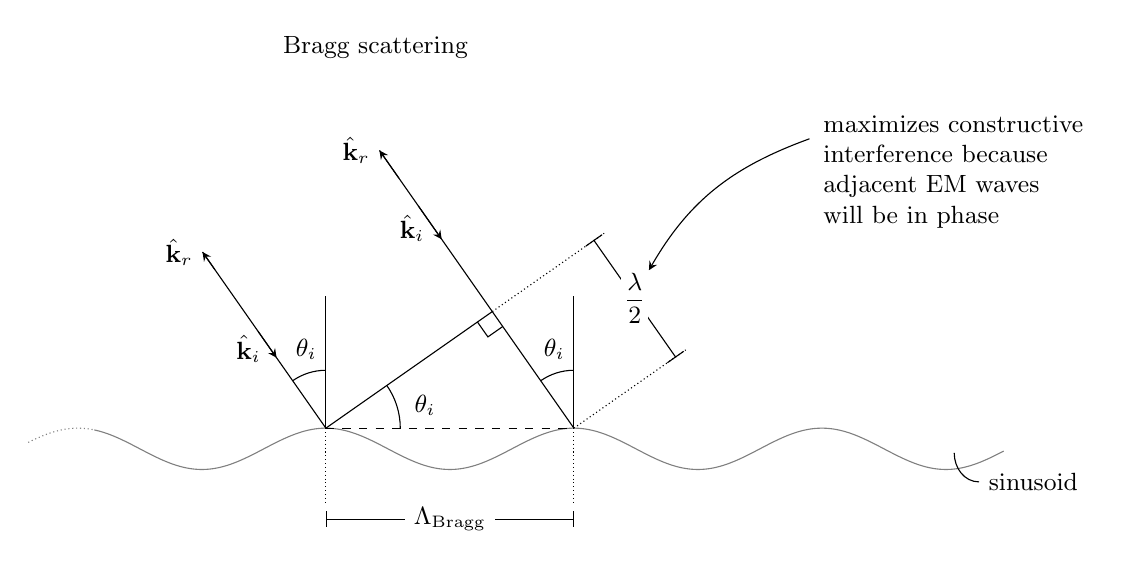
\begin{tikzpicture}[>=stealth, font=\small, scale=1.05]
		\def\ti{35}\def\LB{3}
		\pgfmathsetmacro{\s}{sin(\ti)}\pgfmathsetmacro{\c}{cos(\ti)}
		\node at (0.6,4.6) {Bragg scattering};
		% surface: crests at x = 0 and x = 3
		\draw[densely dotted, gray] plot[domain=-3.6:-2.8, samples=30, smooth] (\x,{0.25*cos(deg(2*pi*\x/\LB))-0.25});
		\draw[gray] plot[domain=-2.8:8.2, samples=200, smooth] (\x,{0.25*cos(deg(2*pi*\x/\LB))-0.25});
		\draw (7.6,-0.3) to[out=-90,in=180] (7.9,-0.65) node[right] {sinusoid};
		% normals
		\foreach \xc in {0,\LB} {
			\draw (\xc,0) -- (\xc,1.6);
			\draw[densely dotted] (\xc,0) -- (\xc,-0.9);
		}
		\draw[dashed] (0,0) -- (\LB,0);
		% left ray (length 2.6) and right ray (length 4.1)
		\coordinate (L0) at ({-2.6*\s},{2.6*\c});
		\coordinate (R0) at ({\LB-4.1*\s},{4.1*\c});
		\draw (L0) -- (0,0);
		\draw (R0) -- (\LB,0);
		\draw[->] ($(0,0)!0.9!(L0)$) -- (L0) node[left] {$\hat{\mathbf{k}}_r$};
		\draw[->] ($(0,0)!0.55!(L0)$) -- ($(0,0)!0.4!(L0)$);
		\node[left] at ($(0,0)!0.45!(L0)$) {$\hat{\mathbf{k}}_i$};
		\draw[->] ($(\LB,0)!0.9!(R0)$) -- (R0) node[left] {$\hat{\mathbf{k}}_r$};
		\draw[->] ($(\LB,0)!0.8!(R0)$) -- ($(\LB,0)!0.68!(R0)$);
		\node[left] at ($(\LB,0)!0.72!(R0)$) {$\hat{\mathbf{k}}_i$};
		% angle arcs at the normals
		\draw (0,0.7) arc (90:{90+\ti}:0.7); \node at ({-0.45*\s+0.02},0.95) {$\theta_i$};
		\draw (\LB,0.7) arc (90:{90+\ti}:0.7); \node at ({\LB-0.45*\s+0.02},0.95) {$\theta_i$};
		% perpendicular from the left crest to the right ray
		\coordinate (F) at ({\LB-\LB*\s*\s},{\LB*\s*\c});
		\draw (0,0) -- (F);
		\coordinate (P1) at ($(F)!0.22cm!(0,0)$); \coordinate (P3) at ($(F)!0.22cm!(\LB,0)$);
		\draw (P1) -- ($(P1)+(P3)-(F)$) -- (P3);
		\draw (0.9,0) arc (0:\ti:0.9); \node at (1.2,0.28) {$\theta_i$};
		% dimension lambda/2 along the right ray, offset toward upper right
		\coordinate (off) at ({\c},{\s});
		\coordinate (Fo) at ($(F)+1.5*(off)$);
		\coordinate (Bo) at ($(\LB,0)+1.5*(off)$);
		\draw[densely dotted] (F) -- ($(Fo)+0.15*(off)$);
		\draw[densely dotted] (\LB,0) -- ($(Bo)+0.15*(off)$);
		\draw (Fo) -- (Bo);
		\draw ($(Fo)+0.12*(off)$) -- ($(Fo)-0.12*(off)$);
		\draw ($(Bo)+0.12*(off)$) -- ($(Bo)-0.12*(off)$);
		\node[fill=white, inner sep=1pt] (lh) at ($(Fo)!0.5!(Bo)$) {$\dfrac{\lambda}{2}$};
		% note
		\node[anchor=west, align=left] at (5.9,3.1) {maximizes constructive\\interference because\\adjacent EM waves\\will be in phase};
		\draw[->] (5.85,3.5) to[out=200,in=60] (lh.north east);
		% Bragg wavelength bar
		\draw[|-|] (0,-1.1) -- node[fill=white] {$\Lambda_\mathrm{Bragg}$} (\LB,-1.1);
	\end{tikzpicture}
	\caption{Geometry of Bragg scattering from a sinusoidal surface of wavelength $\Lambda_\mathrm{Bragg}$ for a wave incident at $\theta_i$. The path to the farther crest is longer by $\Lambda_\mathrm{Bragg}\sin\theta_i = \lambda/2$ each way, so the backscattered waves from adjacent crests differ in path by one EM wavelength and add in phase.}
	\label{f:bragg}
\end{figure}
% NOTE: the caption is an added description.

\begin{itemize}
	% NOTE: handwritten lambda_Bragg, lambda_EM, K_Bragg, K_EM written Lambda_Bragg (D61), lambda, K_Bragg, k (D14).
	% Checked by the geometry of Figure f:bragg (round-trip path difference 2 Lambda_Bragg sin theta_i = lambda) and
	% against van Zyl 2011, Eq. 5.2-4 (p. 199), where W is evaluated at 2k sin theta, and Lecture 7 (backscatter:
	% (k_x, k_y) = (-2k sin theta_i, 0)).
	\item From geometry, we find
	\begin{equation}
		\label{e:LB}
		\Lambda_\mathrm{Bragg} = \frac{\lambda}{2\sin\theta_i}
	\end{equation}
	or
	\begin{equation}
		\label{e:KB}
		K_\mathrm{Bragg} = 2k\sin\theta_i = \frac{2\pi}{\Lambda_\mathrm{Bragg}} \equiv \text{Bragg wavenumber}.
	\end{equation}
\end{itemize}

\subsection{The first-order small-perturbation model}

\begin{itemize}
	% NOTE: checked against van Zyl 2011, Eq. 5.2-4 (p. 199): sigma = 4 pi k^4 h^2 cos^4 theta |alpha|^2 W(2k sin theta)
	% with van Zyl's normalization W_vZ = (2/pi) int r rho J_0 dr (Eq. 5.2-9, p. 200), which is (2/pi) times the W of
	% Lecture 7, Eq. (e:W) (python3, see the Lecture 7 notes); 4 pi (2/pi) = 8, so Eq. (e:spm) agrees. Equivalently,
	% with the two-sided height spectrum Psi = h^2 W/(2 pi) (int Psi d^2K = h^2), Eq. (e:spm) is
	% 16 pi k^4 cos^4 theta |alpha|^2 Psi. Rice (1951) as in van Zyl p. 199.
	\item To apply the concept of Bragg scattering to backscattered power, Rice (1951) applied perturbation methods and derived an expression for the first-order (meaning, higher-order terms in the Taylor series expansion are dropped) normalized radar cross section
	\begin{equation}
		\label{e:spm}
		\sigma_{pp}^0 = 8k^4h^2\cos^4\theta_i\left|\alpha_{pp}\right|^2W\left(K_\mathrm{Bragg},0\right),
	\end{equation}
	where $W(k_x,k_y) \equiv$ surface roughness spectrum discussed in the previous lecture
	% NOTE: checked: Lecture 7, Eq. (e:W_g), W = (ell^2/2) exp{-(k_x^2 + k_y^2) ell^2/4}, at (2k sin theta_i, 0) gives
	% (ell^2/2) exp{-(ell k sin theta_i)^2}.
	\begin{equation}
		\label{e:Wg}
		\left(W = \frac{\ell^2}{2}\exp\left\{-\left(\ell k\sin\theta_i\right)^2\right\} \quad \text{for a Gaussian surface}\right).
	\end{equation}
	\item The scattering coefficients are
	% NOTE: handwritten alpha_pp kept (master table D71). alpha_hh = rho_h (Lecture 5, Eq. for rho_h) equals
	% -alpha_hh of van Zyl 2011, Eq. 5.2-5 (p. 199); only |alpha|^2 enters Eq. (e:spm).
	\begin{equation}
		\label{e:ahh}
		\alpha_{hh} = \rho_h \equiv \text{Fresnel reflection coefficient for $h$-polarized waves at oblique incidence},
	\end{equation}
	% NOTE: handwritten first form reads alpha_vv = -[rho_v + tau_v^2 (eps_2 - 1) tan^2(theta_i)/(2 eps_2)]; corrected
	% to rho_v - tau_v^2 (eps_2 - 1) tan^2(theta_i)/2 because, with rho_v and tau_v as defined in Lecture 5
	% (rho_v = (eta_2 cos theta_t - eta_1 cos theta_i)/(eta_2 cos theta_t + eta_1 cos theta_i),
	% tau_v = 2 eta_2 cos theta_i/(...)), the handwritten form disagrees with the closed
	% form (second line, which is correct) at every angle; e.g., at theta_i = 0 it gives -rho(0) instead of
	% alpha_vv(0) = alpha_hh(0) = rho(0), which symmetry requires. The corrected form equals the closed form exactly
	% (python3, eps_2 = 3, 10 - 2j, 56.2 - 37.4j; theta_i = 10--80 deg). The handwritten form holds in a convention with
	% the opposite sign of rho_v and a transmission coefficient 1 + rho_v (= sqrt(eps_2) tau_v in Lecture 5's
	% convention). The closed form is -1 times van Zyl 2011, Eq. 5.2-6 (p. 199), consistent with alpha_hh = rho_h.
	\begin{align}
		\alpha_{vv} &= \rho_v - \tau_v^2\,\frac{\left(\varepsilon_2 - 1\right)\tan^2\theta_i}{2} \label{e:avv}\\
		&= \left(\varepsilon_2 - 1\right)\frac{\sin^2\theta_i - \varepsilon_2\left(1 + \sin^2\theta_i\right)}{\left(\varepsilon_2\cos\theta_i + \sqrt{\varepsilon_2 - \sin^2\theta_i}\right)^2}, \nonumber
	\end{align}
	where $\rho_v$ and $\tau_v$ are the Fresnel reflection and transmission coefficients for $v$-pol at oblique incidence (Lecture 5), and we have assumed $\varepsilon_1 \approx 1$.
	% NOTE: added "(Lecture 5)".
\end{itemize}

\subsubsection{Why does $\alpha_{hh} = \rho_h$ but $\alpha_{vv} \ne \rho_v$?}

% NOTE: a precise reason, added as a comment only: the Bragg-resonant roughness in backscatter has its wavevector in
% the plane of incidence (k_y = 0), so its crests run along y, parallel to the h-polarized E field, which is
% therefore exactly tangent to that roughness.
\begin{itemize}
	\item[A.] Go back to EM boundary conditions: recall from Faraday's law we got the condition that the tangential component of the electric field is continuous across the surface (Lecture 4); the $h$ field is entirely tangent to the surface for all roughness (at least to a reasonable approximation), whereas the tangential component of the $v$ field changes with roughness.
	% NOTE: added "(Lecture 4)".
\end{itemize}

\subsubsection{Key take-aways}

\begin{enumerate}
	% NOTE: checked: van Zyl 2011, p. 201 (the single-scattering term predicts no depolarization).
	\item $\sigma_{hv}^0 = \sigma_{vh}^0 = 0$ to first order (higher-order factors introduce small nonzero values of $\sigma_{hv}^0$ (and $\sigma_{vh}^0$), but these are generally negligible as they are in the noise of RS instruments).
	\item $\alpha_{pp}$ represents total scattered power and is
	\begin{enumerate}
		\item polarization-dependent;
		\item a function of dielectric properties and viewing geometry (indirectly EM wavelength);
		\item independent of characteristics of surface roughness.
	\end{enumerate}
	\item $W$ influences the direction of scattering and is
	\begin{enumerate}
		\item dependent on characteristics of roughness;
		\item dependent on EM wavelength and viewing geometry;
		\item independent of dielectric properties;
		\item independent of polarization.
	\end{enumerate}
	% NOTE: added "for theta_i > 0 (at normal incidence alpha_vv = alpha_hh)". Checked (python3): |alpha_vv| > |alpha_hh|
	% for eps_2 = 3, 10 - 2j, 56.2 - 37.4j at theta_i = 10--80 deg; cf. van Zyl 2011, Fig. 5-9 (p. 203), where
	% sigma_hh/sigma_vv < 0 dB.
	\item $\sigma_{vv}^0 > \sigma_{hh}^0$ for $\theta_i > 0$ (at normal incidence $\alpha_{vv} = \alpha_{hh}$) due to the expression for reflectivity (thus, due to EM BCs).
\end{enumerate}

%%%%%%%%%%%%%%%%%%%%%%%%%%%%%%%%%%%%%
\section{Tilted Bragg scatter model}
\label{s:tilted}

\begin{itemize}
	\item The previous model only applies to horizontal surfaces with small-scale roughness.
	\item We can combine the Bragg model with the Kirchhoff model for undulating surfaces (Lecture 7) by (again) treating the surface as a bunch of randomly rough surfaces (infinite extent) that are tilted due to longer-wavelength roughness features.
	% NOTE: added "(Lecture 7)".
	\item On the ocean, this simply means that we represent the wind-driven gravity--capillary waves with a Bragg scatter model and rotate our local coordinate system to account for the passage of gravity waves (swells).
	% NOTE: kept as handwritten. U&L 2014, p. 793, give 20--60 deg as the range where Bragg scattering dominates
	% ocean backscatter; van Zyl 2011, p. 198, says facet scattering dominates below 20--30 deg.
	\item This is a very accurate, simple model of scattering from the ocean surface for incidence angles ranging from 30$^\circ$--65$^\circ$. (Lower incidence angles produce primarily specular scatter, while angles $>65^\circ$ involve different mechanisms that we won't discuss in this course because they are esoteric.)
\end{itemize}

\subsection{Normalized radar cross section of a tilted patch}

% NOTE: the handwritten anti-plane tilt symbol is the same glyph as the Lecture 7 surface height (typeset xi there);
% written zeta here to distinguish the tilt from the surface height xi(x,y) (instructor decision, master table D72).
% psi (in-plane tilt) is new and has no clash in the master table.
\begin{itemize}
	\item If we define the tilting of the rough surface patches in terms of two angles
	\begin{itemize}
		\item $\psi \equiv$ in-plane (plane of incidence) tilt,
		\item $\zeta \equiv$ anti-plane (plane of incidence) tilt,
	\end{itemize}
	it can be shown (Valenzuela, 1978) that the normalized radar cross section is
	% NOTE: handwritten reads sigma_pq^0 = 8 K_EM^4 h^2 cos^4(theta_i) Gamma_pq W; cos^4 theta_i corrected to
	% cos^4 theta_i' (local angle of incidence, handwritten theta_m) by derivation: the model applies the first-order
	% result, Eq. (e:spm), in the local frame of the tilted patch, where the angle of incidence is theta_i', so the
	% cos^4 factor, like the Bragg wavenumber |K| = 2k sin theta_i' below, is evaluated at the local angle; the two
	% angles in general differ (they agree, e.g., when psi = zeta = 0). Evidence: derivation, and van Zyl 2011, p. 199,
	% below Eq. 5.2-4: theta there "is the local incidence angle at which the radar waves impinge on the surface", and
	% local slopes change the local incidence angle. For the same reason alpha_hh and alpha_vv are evaluated at
	% theta_i' (added below).
	\begin{equation}
		\label{e:tilt}
		\sigma_{pq}^0 = 8k^4h^2\cos^4\theta_i'\,|S_{pq}|^2\,W,
	\end{equation}
	where
	% NOTE: checked (python3): the magnitude of this argument is 2k sin theta_i', the tangential part of the
	% backscatter Bragg vector -2k k_hat_i on the tilted patch. The split into two components depends on the choice
	% of local axes and was not verified separately (for an isotropic W only the magnitude matters).
	\begin{equation}
		\label{e:Wtilt}
		W = W\big(2k\sin(\theta_i + \psi),\ 2k\cos(\theta_i + \psi)\sin\zeta\big),
	\end{equation}
	and the polarization-dependent reflectivities, written as squared magnitudes of the rotated scattering coefficients $S_{pq}$, are
	% NOTE: handwritten Gamma_pq written |S_pq|^2 (D73) and "written as ... S_pq" added; handwritten theta_m
	% written theta_i' (D74). Checked by
	% derivation (python3, explicit vectors): the local h-polarization vector (k_hat_i x local normal) is rotated
	% from the global one by an angle beta with cos beta = sin(theta_i + psi) cos zeta/sin theta_i' and
	% sin beta = sin zeta/sin theta_i'; rotating the local scattering matrix diag(alpha_hh, alpha_vv) into the global
	% basis (van Zyl 2011, Eq. 4.2-27, p. 160) gives S_pp = cos^2 beta alpha_pp + sin^2 beta alpha_qq and
	% S_hv = sin beta cos beta (alpha_vv - alpha_hh), with Gamma_pq = |S_pq|^2.
	\begin{equation}
		\label{e:Gpp}
		|S_{pp}|^2 = \left|\left(\frac{\sin(\theta_i + \psi)\cos\zeta}{\sin\theta_i'}\right)^2\alpha_{pp} + \left(\frac{\sin\zeta}{\sin\theta_i'}\right)^2\alpha_{qq}\right|^2 \qquad \text{for } p \ne q,
	\end{equation}
	% NOTE: handwritten reads (sin(theta_i + psi) sin xi cos xi/sin theta_m)^2 |alpha_vv - alpha_hh|^2; corrected
	% sin theta_m to sin^2 theta_i' because S_hv = sin beta cos beta (alpha_vv - alpha_hh) and
	% sin beta cos beta = sin(theta_i + psi) sin zeta cos zeta/sin^2 theta_i' (derivation above). The handwritten
	% expression in parentheses equals sin beta cos beta sin theta_i', so it underestimates |S_hv|^2 by the factor
	% sin^2 theta_i' (e.g., theta_i + psi = 30 deg, zeta = 45 deg: 0.316 instead of 0.400 before squaring, python3).
	\begin{equation}
		\label{e:Ghv}
		|S_{hv}|^2 = |S_{vh}|^2 = \left(\frac{\sin(\theta_i + \psi)\sin\zeta\cos\zeta}{\sin^2\theta_i'}\right)^2\left|\alpha_{vv} - \alpha_{hh}\right|^2,
	\end{equation}
	with
	% NOTE: handwritten cos(theta + psi) written cos(theta_i + psi).
	\begin{equation}
		\label{e:thm}
		\theta_i' = \cos^{-1}\big(\cos(\theta_i + \psi)\cos\zeta\big) \equiv \text{incidence angle measured relative to the surface normal},
	\end{equation}
	and $\alpha_{hh}$ and $\alpha_{vv}$ as defined in the Bragg model (Eqs.~\ref{e:ahh} and \ref{e:avv}), evaluated at $\theta_i'$.
	% NOTE: added "(Eqs. ...), evaluated at theta_i'" (see the NOTE at Eq. e:tilt).
\end{itemize}

\subsection{Take-aways}

\begin{itemize}
	\item This model reduces to the previous (untilted) model when $\psi = \zeta = 0$.
	\item Take-aways:
	\begin{itemize}
		\item Tilting modifies both reflectivity and the effective roughness spectrum.
		\item But the dependencies of reflectivity and roughness spectrum remain the same as in the Bragg model and also include tilt angles.
		% NOTE: added "(and theta_i + psi != 0)": by Eq. (e:Ghv), |S_hv|^2 = 0 if sin(theta_i + psi) = 0 even when
		% |zeta| > 0 (the tilt then rotates the polarization basis by 90 deg, swapping h and v).
		\item Cross-polarized scattering ($\sigma_{hv}^0$) is nonzero when the anti-plane tilt angle $|\zeta| > 0$ (and ${\theta_i + \psi \ne 0}$)
		\begin{itemize}
			\item[$\rightarrow$] because in this case, neither the $h$-polarized nor $v$-polarized electric fields are locally tangent to the surface $\Rightarrow$ conservation of the tangential component of the $\mathbf{E}$ field results in a change of polarization.
		\end{itemize}
	\end{itemize}
	\item And those are the basic concepts of EM scattering from surfaces.
\end{itemize}

%%%%%%%%%%%%%%%%%%%%%%%%%%%%%%%%%%%%%
% Symbols follow the master table in ../variables_master.tex; see it for flagged dual usages.
\clearpage
\section*{Variables}

Units are SI. Values are given for universal constants; ``typical'' values are representative, not definitive.

{\small
\renewcommand{\arraystretch}{1.25}
\begin{longtable}{>{$}l<{$} >{\raggedright\arraybackslash}p{0.37\textwidth} >{\raggedright\arraybackslash}p{0.15\textwidth} >{\raggedright\arraybackslash}p{0.24\textwidth}}
\hline
\textrm{Symbol} & Description & Units & Value \\
\hline
\endfirsthead
\hline
\textrm{Symbol} & Description & Units & Value \\
\hline
\endhead
\hline
\endfoot
\multicolumn{4}{l}{\emph{Ocean surface waves}} \\
g & gravitational acceleration & m/s$^2$ & $9.81$ \\
\gamma_\mathrm{st} & surface tension & N/m & $0.0728$ (clean water, 20\textdegree C) \\
\gamma_{\mathrm{st},1},\ \gamma_{\mathrm{st},2} & surface tension of clean water and of surfactant-covered water (Figure 1) & N/m & $0.0728$; $0.035$ (illustrative) \\
\rho_w & mass density of water & kg/m$^3$ & $\approx 1000$ (seawater $\approx 1025$) \\
\omega & angular frequency of an ocean-surface wave & rad/s & -- \\
K & wavenumber of an ocean-surface wave & rad/m & -- \\
\Lambda & wavelength of an ocean-surface wave, $2\pi/K$ & m & gravity: $>2$~cm; capillary: $<2$~cm \\
u_p & phase velocity, $\omega/K$ & m/s & minimum $0.23$ (clean water) \\
h & RMS height of the ocean surface (Sec.~\ref{s:bragg}: of the Bragg-scale roughness) & m & -- \\
\Psi(\omega) & frequency spectrum of the surface height & m$^2$\,s & Eq.~\eqref{e:PM} \\
U & wind speed (19.5~m above the surface in Eq.~\eqref{e:PM}) & m/s & -- \\
\phi_\mathrm{wind} & angle between the plane of incidence and the wind direction & rad & -- \\
A,\ a,\ b,\ n & empirical coefficients in Eq.~\eqref{e:gmf} & varies & inferred from observations \\
\multicolumn{4}{l}{\emph{Bragg scattering}} \\
k & EM angular wavenumber in the medium above the surface & rad/m & $2\pi/\lambda$ \\
\lambda & EM wavelength & m & -- \\
\theta_i & angle of incidence & rad & -- \\
\hat{\mathbf{k}}_i,\ \hat{\mathbf{k}}_r & propagation unit vectors of the incident and backscattered waves & dimensionless & -- \\
\Lambda_\mathrm{Bragg} & Bragg wavelength of the surface roughness & m & $\lambda/(2\sin\theta_i)$ \\
K_\mathrm{Bragg} & Bragg wavenumber & rad/m & $2k\sin\theta_i$ \\
\ell & correlation length & m & -- \\
\sigma_{pq}^0 & normalized radar cross section, receive/transmit polarizations $p$, $q$ & dimensionless & $\sigma_{hv}^0 = 0$ (first order, untilted) \\
W(k_x,k_y) & roughness spectrum (Lecture 7) & m$^2$ & -- \\
k_x,\ k_y & spectral wavenumbers of the roughness spectrum (Lecture 7) & rad/m & -- \\
p,\ q & receive and transmit polarization labels ($h$ or $v$) & -- & -- \\
\alpha_{hh},\ \alpha_{vv} & first-order scattering coefficients & dimensionless & $\alpha_{hh} = \rho_h$ \\
\rho_h,\ \rho_v,\ \tau_v & Fresnel reflection coefficients ($h$, $v$) and transmission coefficient ($v$) & dimensionless & -- \\
\varepsilon_1,\ \varepsilon_2 & dielectric constants above and below the surface & dimensionless & $\varepsilon_1 \approx 1$ \\
\multicolumn{4}{l}{\emph{Tilted Bragg model}} \\
\psi & in-plane tilt of a rough patch (in the plane of incidence) & rad & -- \\
\zeta & anti-plane tilt of a rough patch & rad & -- \\
\theta_i' & local angle of incidence (from the patch normal) & rad & $\cos^{-1}[\cos(\theta_i + \psi)\cos\zeta]$ \\
S_{pq} & rotated scattering coefficient of a tilted patch ($|S_{pq}|^2$: polarization-dependent reflectivity) & dimensionless & $S_{pp} = \alpha_{pp}$ if $\psi = \zeta = 0$ \\
\end{longtable}
}

\end{document}
